\documentclass{article}

\usepackage{ctex}
\usepackage[left=1.25in,right=1.25in,top=1in,bottom=1in]{geometry}
\usepackage{amsmath}
\usepackage{amssymb}
\usepackage{graphicx}
\usepackage{float}
\usepackage{listings}
\usepackage{xcolor}
\lstset{language=Python}   
\lstset{breaklines}              
\lstset{extendedchars=false}
\lstset{ 
	backgroundcolor=\color{white},   % 选择代码背景,必须加上\ usepackage {color}或\ usepackage {xcolor}.
	basicstyle=\footnotesize,        % 设置代码字号.
	breakatwhitespace=false,         % 设置是否当且仅当在空白处自动中断.
	breaklines=true,                 % 设置自动断行.
	captionpos=b,                    % 设置标题位置.
	commentstyle=\color{mygreen},    % 设置注释格式
	deletekeywords={...},            % 是否删除给定语言的关键词.
	escapeinside={\%*}{*)},          % 是否在代码中添加LaTex.
	extendedchars=true,              % 是否允许使用非ASCII字符; 仅适用于8位编码,不适用于UTF-8. 
	frame=single,	                   % 给代码区添加边框.
	keepspaces=true,                 % 保留空格(useful for keeping indentation of code (possibly needs columns=flexible).
	keywordstyle=\color{blue},       % 关键字显示风格.
	language=Octave,                 % 使用的语言.
	morekeywords={*,...},            % 是否需要添加其他的关键词.
	numbers=left,                    % 给代码添加行号,可取值none, left, right.
	numbersep=5pt,                   % 设置行号与代码之间的间隔
	numberstyle=\tiny\color{mygray}, % 行号的字号和颜色
	rulecolor=\color{black},         % 边框颜色,如果没有设置,框架颜色可以在非黑色文本中的换行符上更改(例如 text (e.g. comments (green here)))
	showspaces=false,                % 显示每个地方添加特定下划线的空格; 覆盖了'showtringspaces'
	showstringspaces=false,          % 仅在字符串中允许空格
	showtabs=false,                  % show tabs within strings adding particular underscores
	stepnumber=2,                    % the step between two line-numbers. If it's 1, each line will be numbered
	stringstyle=\color{mymauve},     % string literal style
	tabsize=2,	                   % 将默认tab设置为2个空格
	title=\lstname                   % show the filename of files included with \lstinputlisting; also try caption instead of title
}

\usepackage[framed,numbered,autolinebreaks,useliterate]{mcode}

\author{张泽宇}
\date{2022年4月10日}
\title{第六、七周工作总结}

\begin{document}
	\maketitle
	
	{\centering \rule[15pt]{15cm}{0.1em}}
	
	{
		\noindent
		\large
		\textbf{过去两周的主要进行的工作包括有:
			\begin{itemize}
				\item 学习使用PSCAD,我结合了张正刚师兄给的两个例子,自己搭建了之前的10kV接地小电阻模型,并且逐步进行了完善。
				\item 学会了使用Multiple Run模块进行多重运行,可以自动仿真出多种情况。
				\item 基于python尝试了PSCAD数据接口。
				\item 基于python实现了从一维时间序列到二维灰度图像程序。
			\end{itemize}
		}
		
		以下为详细叙述
		
	{\centering \rule[-10pt]{15cm}{0.1em}}
	
	\newpage
	
	\section{学习使用PSCAD}
	
	相对于Simulink,PSCAD更加专注于电气工程方面的仿真,操作起来也更加的方便。由于网络上相关的教程不是很多,我借助张正刚师兄给的两个例子、PSCAD帮助文档和例程进行了学习,尝试搭建了一个10kV小电阻接地电磁暂态模型,并且进行了逐代完善,将故障发生、多重运行等功能加入。最终的模型如下图所示:
	
	主电路部分如下所示:
	
	\begin{figure}[h]
		\centering 
		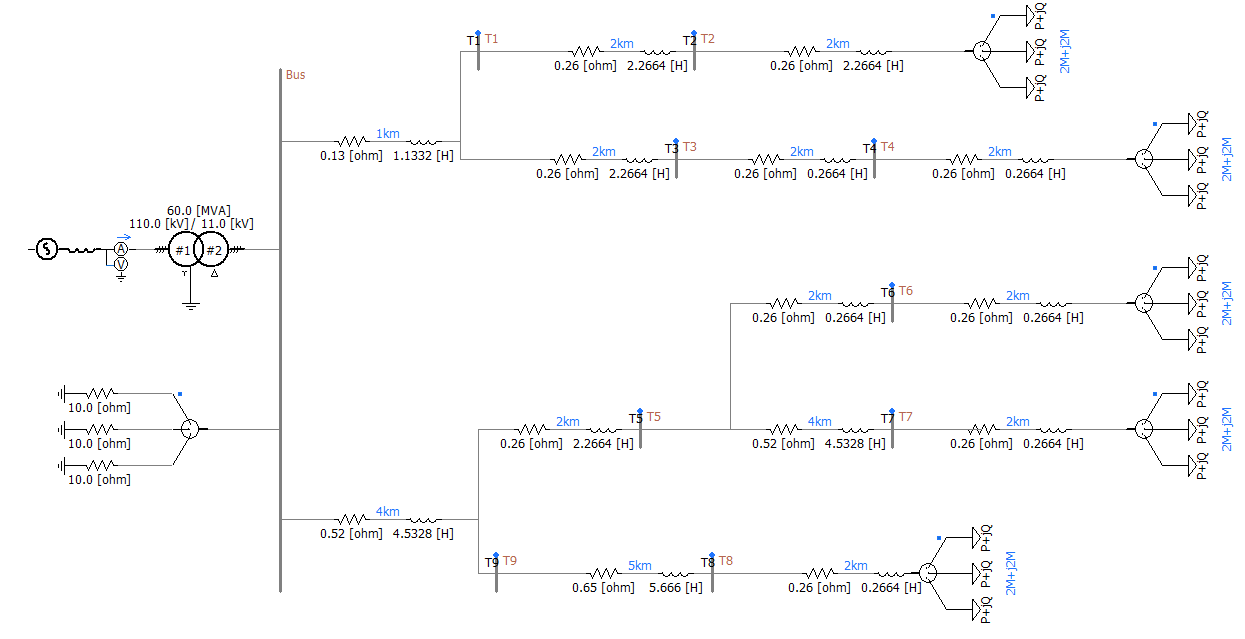
\includegraphics[width=13cm]{figure/1.png}
		\caption{主电路部分}
	\end{figure}

	\begin{figure}[htpb]
		\centering 
		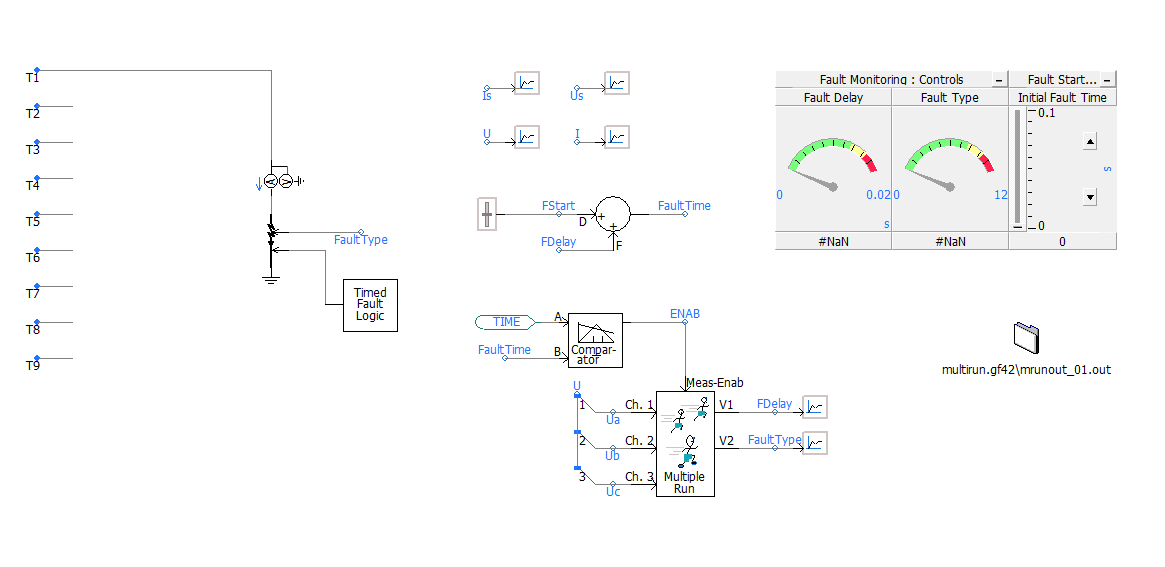
\includegraphics[width=13cm]{figure/2.png}
		\caption{控制部分}
		\label{控制}
	\end{figure}	

	其中三相电压为110kV,频率50Hz接降压变压器,总线上电压为11kV,共有两条馈线,五个负载。负载有功功率2Mw,无功功率2Mw。输电线路用电阻和电感进行等效,每公里单位电阻为0.13$\Omega$,单位电感为1.1332h(这个数据是按照学长给的例子列出来的)。用不同的总线代表不同的故障位置,从T1到T9共有9个故障发生点。
	
	电路的控制部分如下图\ref{控制}所示:
	
	控制部分的左边T1-T9是从主电路上引出的Xnode结点,当模拟不同位置故障发生的时候,只需要在控制部分将Xnode结点与故障发生器连接即可,无需在主电路上进行更改,这样可以便捷布线。
	
	故障发生器由两个输入信号:FaultType控制故障发生的种类,这个数据由Multiple Run元件输入;故障定时控制逻辑元件控制故障时间,其中设置用FaultTime变量表示故障发生时间,故障持续0.02s即一个周期。同时用一个万用表测量故障电流与故障电压,标记为I与U。
	
	中间靠上位置是测量的电源电压、电流和故障电压电流以Data Label形式引出,接输出通道。
	
	中间部分是FaultTime变量的逻辑设置,由起始时间FStart和延迟时间FDelay求和,其中FStart可有右边的Control Panel进行修改,FDelay由Multiple Run元件输入,这样FaultTime就可以表示不同时间段开始,不同滞后时间的故障发生时间。
	
	中间靠下是多重运行的设置。Multiple Run控制两个变量变化,FDelay从0开始,以0.01步长增至0.1;FaultType为列表类型,从1取到10,其中123代表ABC三相短路接地、456代表两相短路接地、7代表三相短路接地、8910代表两相短路。Multiple Run记录三个数据,为故障发生时三相电压。其Meas-Enab通过一个两输入比较器输入,将FaultTime和仿真时间进行比较,控制启用记录数据。
	
	右边上部是控制面板,可以看出当前的FaultTime和FaultType,并可以对FStart进行修改;下部为记录数据。
	
	\begin{figure}[htpb]
		\centering 
		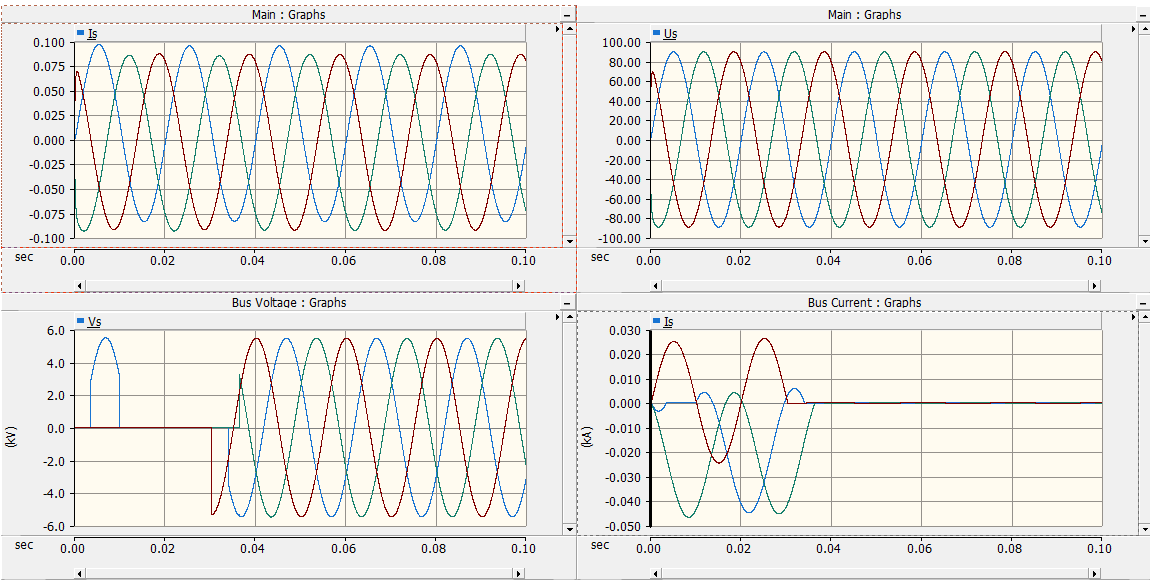
\includegraphics[width=12cm]{figure/3.png}
		\caption{控制部分}
	\end{figure}
	
	电路的显示部分如下图所示:

	通过Graph Pane显示电源电压电流和故障电压电流。
	
	可以看出,增加了Multiple Run之后,每次运行都可以自动多次运行仿真,每次具有不同的参数设置。这极大的增加了数据集的数量。例如,上面的设置中,只要运行一次,就可以得到10*10=100次仿真数据;理论上讲,增多FDelay可以取到的值,是可以将数据数量进一步拓展的,但是否会对电脑性能提出要求,还需要进行尝试。
	
	但是这里还有一个问题,就是电源处三相电流不对称。有一相电流显然较高。这个地方还需要进一步排查原因。
	
	\section{Python数据接口尝试}
	
	在PSCAD上,记录数据有两种途径,一种是通过仿真设置里勾选存储数据的选项,得到.out文件;另一种是通过上面的File Reference存储。
	
	第一种得到的.out文件由数据文件和目录文件组成,如下:
	
	\begin{figure}[htpb]
		\centering 
		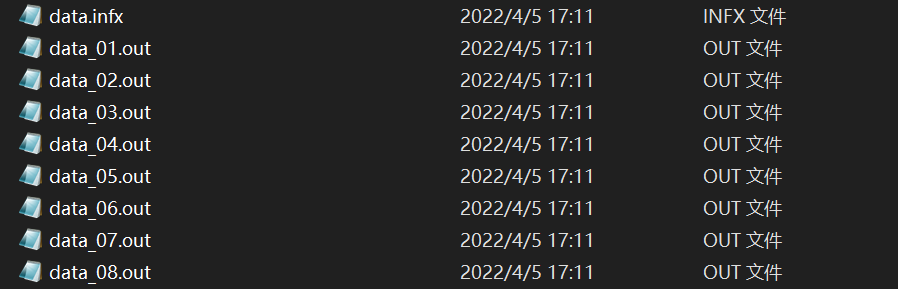
\includegraphics[width=12cm]{figure/4.png}
		\caption{.out文件}
	\end{figure}

	因此基于python,用正则表达式从目录文件提取信息,将数据文件中的数据匹配进去,即可得到最后的数据集。
	
	部分目录文件如下所示:
	\begin{lstlisting}
	<Output device="EMTDC" version="2010" date="2022/04/05" time="17:11:48.000000">
	<Domain name="Time" unit="s" mult="0.0" skew="0.0">
	<Sample rate="100000.0" end="10000" />
	</Domain>
	<List classid="Analog">
	<Analog name="Main(0):Is" index="0" id="1763691693:0" label="" dim="3" unit="" min="-2.0" max="2.0" />
	<Analog name="Main(0):Us" index="3" id="1026695447:0" label="" dim="3" unit="" min="-2.0" max="2.0" />
	<Analog name="Main(0):I1" index="6" id="862159365:0" label="" dim="3" unit="" min="-2.0" max="2.0" />
	\end{lstlisting}

	代码如下:
	\begin{lstlisting}
	import numpy as np
	import re
	
	
	def read_variable_name(f_name):
		L = []
		f = open(f_name, 'r', encoding='utf-8')
		for line in f:
			reformat = re.compile(r'Main\(0\):(.*?)"', re.S)
			index = reformat.finditer(line)
			for item in index:
				L.append(item.group()[8:-1])
		f.close()
		return L
	
	
	def read_variable_time(f_name):
		f = open(f_name, 'r', encoding='utf-8')
		L = []
		for line in f:
			line = line.replace("\n", '')
			line = re.split(r"[ ]+", line)
			if line[1]:
			L.append(line[1])
		else:
			continue
		f.close()
		return L
	
	
	def read_variable_value(f_name):
		f = open(f_name, 'r', encoding='utf-8')
		L_A, L_B, L_C = [], [], []
		for line in f:
			line = line.replace("\n", '')
			line = re.split(r"[ ]+", line)
			if line[1]:
				L_A.append(line[2])
				L_B.append(line[3])
				L_C.append(line[4])
			else:
				continue
		L_A_mat = np.array(L_A)
		L_B_mat = np.array(L_B)
		L_C_mat = np.array(L_C)
		L = np.dstack([L_A_mat, L_B_mat, L_C_mat])
		f.close()
		return L
	
	
	if __name__ == '__main__':
		path_variable_name = "data\\data.infx"
		path_variable = "data\\data_01.out"
		variable_list = read_variable_name(path_variable_name)
		variable_time = read_variable_time(path_variable)
		variable_value = read_variable_value(path_variable)
		print(variable_value)
	\end{lstlisting}

	这份代码还不能作为做中的版本,因为在一些普适性和代码优化方面的工作还没有进行。待完善后就可以拿来直接使用。
	
	对于第二种数据的记录方式,目前得到的数据结果是这样的:
	
	\begin{figure}[htpb]
		\centering 
		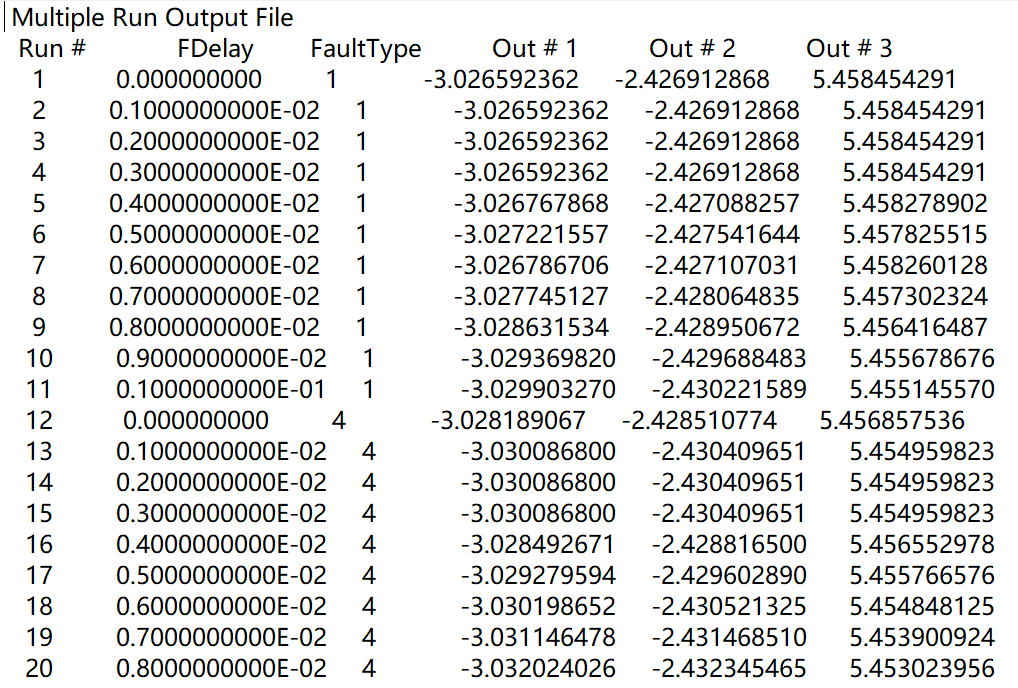
\includegraphics[width=12cm]{figure/7.png}
		\caption{.out文件}
	\end{figure}
	
	目前的数据形式不是我想要的数据形式。如何能够将每个时刻的三相电压输出值写入文件,还需要进行进一步的探究。
	
	\section{从一维时间序列到二维灰度图像转变}
	
	在与陈浩泳师兄交流后,因为CNN更多的优势是体现在图像识别上,我计划先采用将仿真得到的一维时间序列转换为二维灰度图像作为CNN输入的方法。所以这个星期先将时间序列到灰度图的程序进行了编写。
	
	我从网上找到一组一维数据,数据长度为25万左右。随机选择500个起始点,每个起始点往后4096个数据进行堆叠,得到灰度图。
	
	具体代码如下:
	
	\begin{lstlisting}
		import numpy as np
		import random
		import re
		import imageio
		import matplotlib.pyplot as plt
		
		
		def load_data(filename):
			data = []
			file = open(filename, 'r', encoding='utf-8')
			for line in file:
				line = line.replace("\n", '')
				line = re.split(r"[ ]+", line)
				if line[data_column]:
					data.append(eval(line[data_column]))
				else:
					continue
			file.close()
			return data
		
		
		def turn_grayscale(data):
			lens = len(data)
			max_start = lens - dimension_grayscale**2
			starts = []
			gray_scales = []
			for i in range(sampling_value):
				while True:
					start = random.randint(0, max_start)
					if start not in starts:
						starts.append(start)
						break
			temp = data[start: start + dimension_grayscale**2]
			temp = np.array(temp)
			gray_temp = temp.reshape(dimension_grayscale, dimension_grayscale)
			gray_scales.append(gray_temp)
			return gray_scales
		
		
		def draw_grayscale(graydata):
			np.savez(name_npz, *graydata)
		
		
		def npz_visualization(filename):
			npz_file = np.load(filename, allow_pickle=True)
			for file in npz_file:
				temp = npz_file['{}.npy'.format(file)]
				plt.imshow(temp)
				imageio.imwrite("depth.jpg", temp)
				plt.savefig('temp.jpg')
				plt.show()
				break
			return
		
		
		def divide_dataset(filename):
			npz_file = np.load(filename, allow_pickle=True)
			for file in npz_file:
				temp = npz_file[file]
				imageio.imwrite("DataSet\\{}.jpg".format(file), temp)
			return
		
		
		if __name__ == '__main__':
			dimension_grayscale = 64
			data_column = 0
			sampling_value = 500
			name_npz = 'grayscales'
			DataSet = load_data('data.txt')
			graydata_temp = turn_grayscale(DataSet)
			draw_grayscale(graydata_temp)
			# npz_visualization('graydatas.npz')
			divide_dataset(name_npz + '.npz')
			print('success!')
	\end{lstlisting}
	
	转化成的灰度图像如下所示:
	
	\begin{figure}[htpb]
		\centering 
		
\includegraphics[width=6cm]{figure/8.jpg}
		\caption{灰度图像}
	\end{figure}
	
	我昨天也与陈师兄进行了交流,目前等他将数据仿真出来,先简单的用CNN测试一下,建立闭环,验证可行性,然后再考虑完善结果。
	
	以上即为我上两周进行的主要工作。
\end{document}
